%% HEADER
%%%%%%%%%%%%%%%%%%%%%%%%%%%%%%%%%%%%%%%%%%%%%%%%%%%%%%%%%%%%%
\newcommand{\hyperrefpdfauthor}{}
\newcommand{\hyperrefpdftitle}{}
\newcommand{\hyperrefpdfsubject}{}
\newcommand{\hyperrefpdfkeywords}{}
\newcommand{\hyperrefpdfborder}{0}
\documentclass{wissdoc-kw-eng}

\newcommand{\eg}[0]{e.g., }
\newcommand{\ie}[0]{i.e., }
\newcommand{\etal}[0]{et~al.}
\newcommand{\floatwidth}[0]{\columnwidth}
\newcommand{\subfloatwidth}[0]{0.48\columnwidth}
\newcommand{\comment}[1]{}
\definecolor{Orange}{rgb}{1,0.5,0}
\newcommand{\todo}[1]{\textsf{\textbf{\textcolor{Orange}{[[#1]]}}}}

\usepackage{tikz}
\usetikzlibrary{decorations.pathmorphing,calc,shapes,shapes.geometric,patterns,snakes,matrix}

\usepackage{dcolumn}
\newcolumntype{d}[1]{D{.}{.}{#1}}

\usepackage[printonlyused]{acronym}
\renewcommand{\bflabel}[1]{\normalfont{\normalsize{#1}}\hfill} % keine serifenlose schrift für acronym
%\usepackage{acronym}
\usepackage{subfigure}

\usepackage{float}
\floatstyle{ruled}
\newfloat{listing}{htbp}{lop}[chapter]
\floatname{listing}{Listing}

\usepackage[hang,center,nooneline]{caption}
\captionsetup[figure]{font={small,sf}}
\captionsetup[table]{font={small,sf}}
\captionsetup[listing]{font={small,sf}}
\usepackage{etoolbox}


%% Normales LaTeX oder pdfLaTeX? %%%%%%%%%%%%%%%%%%%%%%%%%%%%
%% ==> Das neue if-Kommando "\ifpdf" wird an einigen wenigen
%% ==> Stellen benötigt, um die Kompatibilität zwischen
%% ==> LaTeX und pdfLaTeX herzustellen.
%\newif\ifpdf
%\ifx\pdfoutput\undefined
%    \pdffalse              %%normales LaTeX wird ausgeführt
%\else
%    \pdfoutput=1
%    \pdftrue               %%pdfLaTeX wird ausgeführt
%\fi


%% Fonts für pdfLaTeX %%%%%%%%%%%%%%%%%%%%%%%%%%%%%%%%%%%%%%%
%% ==> Nur notwendig, falls keine cm-super-Fonts installiert
\ifpdf
	\usepackage{ae}       %%Benutzen Sie nur eines dieser Pakete:
	%\usepackage{zefonts}  %%je nachdem, welches Sie besitzen.
\else
	%%Normales LaTeX - keine speziellen Fontpackages notwendig
\fi


%% Deutsche Anpassungen %%%%%%%%%%%%%%%%%%%%%%%%%%%%%%%%%%%%%
%\usepackage[T1]{fontenc}
%\usepackage[utf8]{inputenc}

%% zur Zitaten des Quelltextes%%%%%%%%%%%%%%%%%%%%%%%%%%%%%%%
% "final" forces printing of all listings, even if the global "draft" is set
\usepackage[final]{listings}
\lstset{
    basicstyle=\footnotesize\ttfamily,
    tabsize=4,
    numberstyle=\tiny\color{gray},
    numbersep=5pt,
    numbers=left,
    captionpos=b,
    abovecaptionskip=0pt,
    belowcaptionskip=0pt,
    aboveskip=10pt,
    belowskip=0pt,
    floatplacement=tbp,
    frame=topline,
    framerule=.1pt,
    framesep = 3pt,
    }
\renewcommand\lstlistingname{\textbf{Listing}}
% This is only kept for backwards compatibility. You should never have to use it. Use the listing-environment instead.
%\DeclareCaptionFormat*{lstruled}{{\bfseries#1\small\space\normalfont#3\hrule height.1pt depth0pt}\par}
%\captionsetup[lstlisting]{format=lstruled,singlelinecheck=false}

%% mehrere Abbildungen in eine %%%%%%%%%%%%%%%%%%%%%%%%%%%%%%
\usepackage{subfigure}

%% Packages für Formeln %%%%%%%%%%%%%%%%%%%%%%%%%%%%%%%%%%%%%
\usepackage{amsmath}
\usepackage{amsthm}
\usepackage{amsfonts}

%% Zeilenabstand %%%%%%%%%%%%%%%%%%%%%%%%%%%%%%%%%%%%%%%%%%%%
\usepackage{setspace}
%\singlespacing        %% 1-zeilig (Standard)
%\onehalfspacing       %% 1,5-zeilig
%\doublespacing        %% 2-zeilig


%% Andere Packages %%%%%%%%%%%%%%%%%%%%%%%%%%%%%%%%%%%%%%%%%%
%\usepackage{a4wide} %%Kleinere Seitenränder = mehr Text pro Zeile.
\usepackage{fancyhdr} %%Fancy Kopf- und Fußzeilen
%\usepackage{longtable} %%Für Tabellen, die eine Seite überschreiten
\usepackage{lscape}
\usepackage{rotating} 
%\usepackage[htt]{hyphenat} %Trennung von Typewriter-Schriften
%\usepackage{listings}
\usepackage{pstricks-add}


% Tabellen mit Center und left
\usepackage{tabularx,colortbl} % colored table background
\newcolumntype{C}[1]{>{\centering\arraybackslash}p{#1}}
\newcolumntype{R}[1]{>{\raggedleft\arraybackslash}p{#1}}
% Table spacings
\newcommand\T{\rule{0pt}{2.5ex}\rule[-1.0ex]{0pt}{0pt}}
\newcommand\B{\rule[-1.0ex]{0pt}{0pt}}

\definecolor{slightgray}{gray}{.90}
\colorlet{slightred}{red!10}
\colorlet{slightgreen}{green!10}
\colorlet{slightblue}{blue!10}
\colorlet{moteblue}{blue!60!black!20}
\colorlet{motered}{red!60!black!20}

%% Definitionen %%%%%%%%%%%%%%%%%%%%%%%%%%%%


%% zur Benutzung bei ergänzenden Daten%%%%%%%%%%%%%%%%%%%%%%%%
%\usepackage{endnotes}
%\renewcommand{\notesname}{Konfigurationsdaten der Messreihen}
%\renewcommand{\theendnote}{\Alph{endnote}}
%\renewcommand{\enotesize}{\normalsize}

%\hyphenation{Sensor-netz-werk
%}

%%%%%%%%%%%%%%%%%%%%%%%%%%%%%%%%%%%%%%%%%%%%%%%%%%%%%%%%%%%%%
%% DOKUMENT
%%%%%%%%%%%%%%%%%%%%%%%%%%%%%%%%%%%%%%%%%%%%%%%%%%%%%%%%%%%%%
\begin{document}

%% Dateiendungen für Grafiken %%%%%%%%%%%%%%%%%%%%%%%%%%%%%%%
%% ==> Sie können hiermit die Dateiendung einer Grafik weglassen.
%% ==> Aus "\includegraphics{titel.eps}" wird "\includegraphics{titel}".
%% ==> Wenn Sie nunmehr 2 inhaltsgleiche Grafiken "titel.eps" und
%% ==> "titel.pdf" erstellen, wird jeweils nur die Grafik eingebunden,
%% ==> die von ihrem Compiler verarbeitet werden kann.
%% ==> pdfLaTeX benutzt "titel.pdf". LaTeX benutzt "titel.eps".
%\ifpdf
%    \DeclareGraphicsExtensions{.pdf,.jpg,.png}
%\else
%    \DeclareGraphicsExtensions{.eps}
%\fi

\pagestyle{empty} %%Keine Kopf-/Fusszeilen auf den ersten Seiten.

\ifnotdraft{
%% Deckblatt %%%%%%%%%%%%%%%%%%%%%%%%%%%%%%%%%%%%%%%%%%%%%%%%
\frontmatter
\titlehead{
	\centering
	
\includegraphics[height=20mm,keepaspectratio]{thesis-tex/logos/comsys-text}
	\hfill
	
\includegraphics[height=20mm,keepaspectratio]{thesis-tex/logos/rwth}
} % end titlehead

\begin{titlepage}

\let\footnotesize\small \let\footnoterule\relax

\hbox{}
\vfill

\centering

\begin{doublespace} 
{ \huge\textbf{\textsf{Temperature Dependency \\ \vspace{-0.4em}
of Bit Error Distributions \\ \vspace{-0.4em}
in Wireless Sensor Networks \\ \vspace{-0.4em}}}}
\end{doublespace}
\vskip 2cm

{\large Bachelor Thesis\\[5pt]}
{\large \textbf{Niklas Hauser}}
\vskip 1cm

\textbf{RWTH Aachen University, Germany\\[5pt]
        Chair of Communication and Distributed Systems}
\vskip 2cm

\large

Advisors:
\vskip 2mm

\begin{tabular}{R{7cm}p{7cm}}
Dr. & Matteo Ceriotti\\
Dipl.-Inform. & Florian Schmidt\\
Prof.~Dr.-Ing. & Klaus Wehrle\\
Prof.~Dr.~rer.~nat. & Bernhard Rumpe
\end{tabular}
\vskip 1cm

\begin{tabular}{R{6cm}p{6cm}}
Registration date:  & January 29, 2014 \\
Submission date:    & May 29, 2014 \\
\end{tabular}

\vfill

\end{titlepage}


\cleardoublepage
\thispagestyle{empty}
\vspace*{36\baselineskip}
\hbox to \textwidth{\hrulefill}

I hereby affirm that I composed this work independently and used no other than the specified sources and tools and that I marked all quotes as such.

Hiermit versichere ich, dass ich die Arbeit selbstständig verfasst und keine anderen als die angegebenen Quellen und Hilfsmittel benutzt sowie Zitate kenntlich gemacht habe.

Aachen, den 29. Mai 2014

\cleardoublepage
\cleardoublepage

% \selectlanguage{german}

\begin{center}
\paragraph{Kurzfassung}
\hrulefill

\end{center}

Mit der Verfügbarkeit von leistungsfähigen eingebetteten Geräten und kostengün\-stigen Funkmodulen, beginnen auch immer mehr batteriebetriebene Sensorgeräte miteinander zu reden und Probleme gemeinsam zu entscheiden.
Es ist abzusehen, dass die Benutzung solcher intelligenten Geräte in drahtlosen Sensornetzwerken in\-dustrielle Prozesse vereinfachen und unsere Lebensqualität verbessern wird.

Allerdings ist die Laufzeit dieser mobilen Geräte durch ihre endliche Energiequelle, die meist nur mit viel Aufwand zu wechseln ist, beschränkt. Daher braucht es eine Programmierung, die energiebewusst kommuniziert, um die Lebensdauer der Bat\-terie so weit wie möglich zu verlängern.
Drahtlose Kommunikation ist stark durch Umweltveränderungen, allen voran die Lufttemperatur, beinflussbar, was zu Korrup\-tion oder Verlust von Paketen führen kann und ein erneutes Versenden des Pakets nach sich zieht.

In dieser Arbeit beschreiben wir eine kostengünstige Testplatform zum Testen der Funkverbindungen in einer temperaturkontrollierten Umgebung. Mit dieser Plat\-form untersuchen wir die Empfangsraten und die Bitfehlerverteilungen in korrupten Paketen.
Unsere Ergebnisse widerlegen frühere veröffentlichte Ergebnisse.
Schließ\-lich wenden wir diese Erkenntnisse auf die Programmierung eines Simulators an, mit dem wir untersuchen, wie sich Temperatur als Eingabegröße einer adaptiven Vorwärtsfehlerkorrektur verhält, um damit die Empfangsraten korrupter Pakete zu verringern.

% \selectlanguage{english}

\vspace {0.5cm}
\begin{center}
\paragraph{Abstract}
\hrulefill
\end{center}

With the availability of powerful embedded devices and inexpensive radio communication, ever more battery powered sensor devices make use of the added connectivity to talk to each other and decide problems collectively.
It is envisioned that usage of such smart devices in \acl{WSN}s will streamline industrial processes as well as improve our quality of life.

However, the runtime of these mobile devices is limited by their finite power source, which most often are impractical to exchange.
Therefore energy-aware programming and communication is required to prolong battery life for as long as possible.
Unfortunately, wireless communication is strongly influenced by environmental changes, most prominently air temperature, which can lead to packet corruption or loss and requires energy-consuming retransmissions.

In this work we describe a low-cost testbed for testing radio performance in a temperature-controlled environment, with which we examine packet reception rates and bit error distributions within packet corruption. Our results disprove previous published findings.
Finally, we apply these findings on building a simulator, with which we investigate using temperature as an input for an adaptive \acl{FEC} scheme to improve packet reception rates and thereby reduce unnecessary retransmissions.

\cleardoublepage
\cleardoublepage

\chapter*{Acknowledgments}



\cleardoublepage

% Titelseite hatte noch normale Tabellen. Von hier ab sollen alle
% Tabellen laut style-Vorgaben sans serif sein.
\AtBeginEnvironment{tabular}{\sffamily}
\AtBeginEnvironment{tabularx}{\sffamily}

%% Inhaltsverzeichnis %%%%%%%%%%%%%%%%%%%%%%%%%%%%%%%%%%%%%%%
\tableofcontents %Inhaltsverzeichnis
\cleardoublepage %Das erste Kapitel soll auf einer ungeraden Seite beginnen.
} % end ifnotdraft

\pagestyle{fancy} %%Ab hier die Kopf-/Fusszeilen: headings / fancy / ...

%%%%%%%%%%%%%%%%%%%%%%%%%%%%%%%%%%%%%%%%%%%%%%%%%%%%%%%%%%%%%
% einzelne Kapitel
%%%%%%%%%%%%%%%%%%%%%%%%%%%%%%%%%%%%%%%%%%%%%%%%%%%%%%%%%%%%%
%\include{commands}

\mainmatter
\chapter{Introduction}



\chapter{Testbed Description}

\section{Temperature Box}

Even though previous setups used an infrared lamp~\cite{Boano2013, Hermans2013} to heat the motes directly, we chose to control mote temperature sorely using air temperature.
The mote is placed in a closed styrofoam box and the confined air is heated to the requested temperature and circulated to transfer this heat to the mote.

\subsection{Hardware}
A microcontroller evaluates temperature sensors within the box and locally controls the duty cycles of the PC fan and 150W ceramic heating element using a PID loop to achieve the requested air temperature.
The controller is equipped with a serial connection to be used to set the desired temperature and read out the actual temperature.

Additionally air temperature is displayed as a hue from blue (cold) via green (warm) to red (hot) by an RGB LED and the duty cycles of the heating element and fan are mapped to two white LEDs, to provide an immidiate heating system overview and prevent burn injuries.

The box is powered by an ATX power supply, chosen for its wide availibility and the ability to provide 12V, 5V and 3.3V at the required currents, which removes the need for additional (costly) voltage conversion.
A custom designed PCB distibutes power from the ATX connectors to two high and two medium power MOSFET switches and up to four temperature sensors, all controlled by an ATmega328p.

The PCB, heating element and fan are fastened using holders on a baseplate, which were prototyped using the PCB mill and lasercutter of the RWTH FabLab~\cite{fablab}.
The styrofoam box has the outside dimensions of $35 \times 35 \times 30$cm with a wall thickness of 5cm which results in a holding capacity of $12.5\ell$.

Picture~\ref{pic:box_hardware} shows the controller, heating element, fan and mote harness.

\subsection{Embedded Software}

The embedded software is written using the xpcc microcontroller framework~\cite{xpcc.io} and implemented as a set of asynchronous control tasks for input parsing and output formatting, temperature sensor evaluation, PID loop update and duty cycle generation.
All switching frequencies were kept as low as possible to avoid any interference with the 2.4GHz band.

\subsection{Evaluation}

The heating element has enough power to create air temperatures of up to $120\,^{\circ}\mathrm{C}$, however, a limit of $90\,^{\circ}\mathrm{C}$ is imposed during experiments, since the mote is only rated up to $85\,^{\circ}\mathrm{C}$ and the styrofoam starts to break apart.
As seen in Figure~\ref{fig:box_heating_cooling} it takes about 40 minutes to heat up to $90\,^{\circ}\mathrm{C}$ and more than 2 hours to cool back down to $30\,^{\circ}\mathrm{C}$.

During the experiments a stepping heating approach is used similar to Figure~\ref{fig:box_heating_step}.

With a room temperature of $20-25\,^{\circ}\mathrm{C}$, the minimum experiment temperature was set at $30\,^{\circ}\mathrm{C}$ so that it can be reached within reasonable time.
The boxes can be retrofitted with an active piezoelectric cooling element and a fan by connceting them to the two unused MOSFET switches on the controller and updating the software.

\begin{figure}[t]
	\centering
    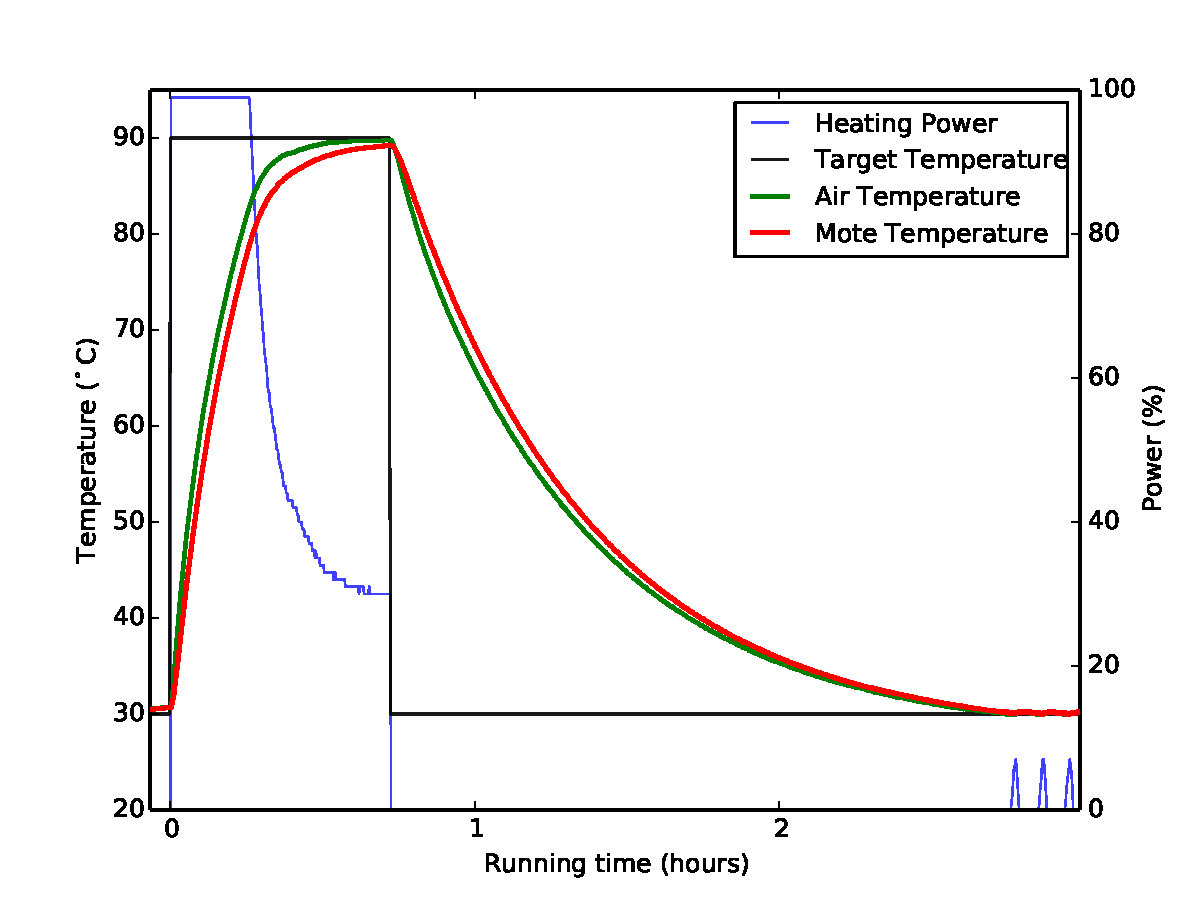
\includegraphics[width=1\columnwidth]{figures/box_heating_cooling}
	\caption{Temperature box heating up to $90\,^{\circ}\mathrm{C}$, then cooling back down to $30\,^{\circ}\mathrm{C}$.}
    \label{fig:box_heating_cooling}
\end{figure}

\begin{figure}[t]
	\centering
    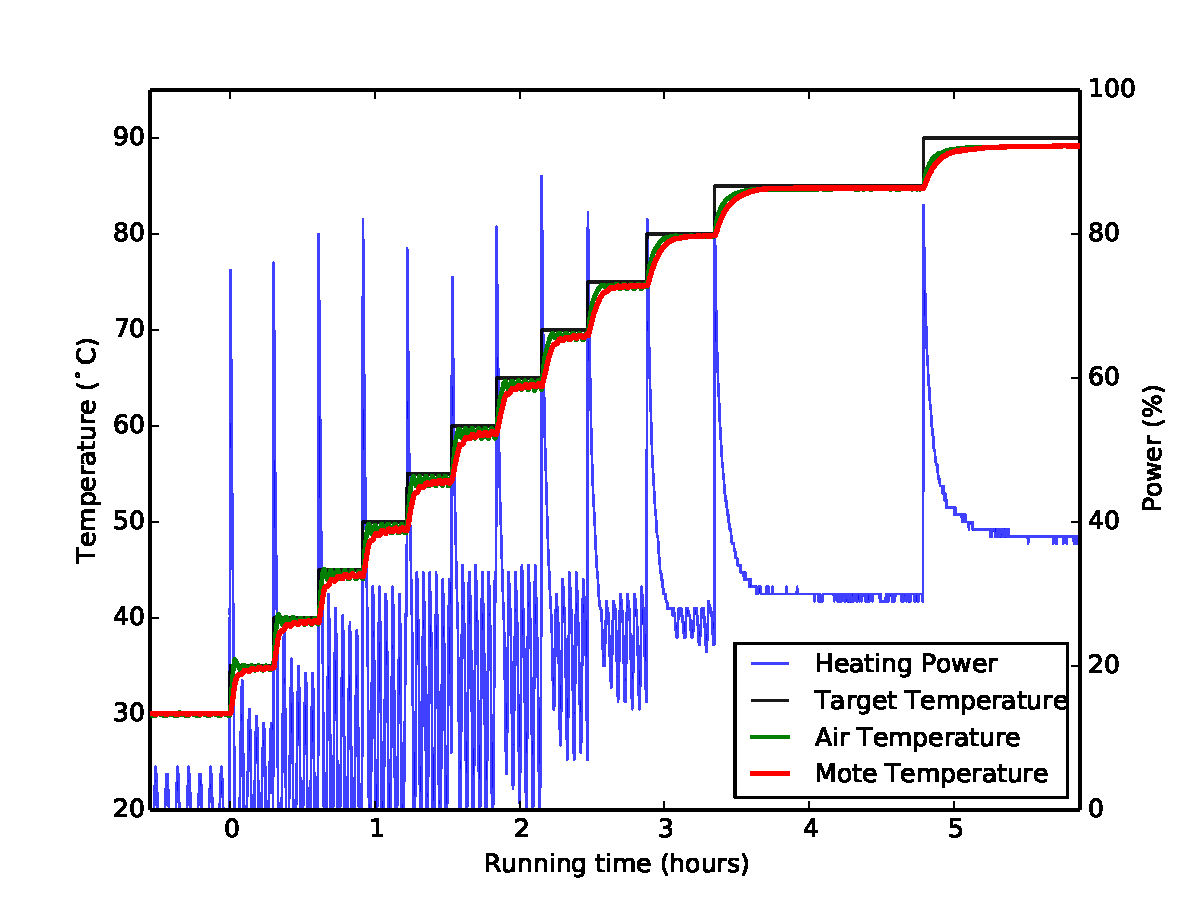
\includegraphics[width=1\columnwidth]{figures/box_heating_step}
	\caption{Typical experiment setup with temperature increases in steps of $5\,^{\circ}\mathrm{C}$.}
    \label{fig:box_heating_step}
\end{figure} 
\chapter{Experiments}

Several experiment setups were designed to focus on the effect of temperature on the mote hardware and link quality.
All experiments were done using the on-board PCB antenna, sending on channel 26 to minimize WiFi interference.

\section{Clock Drift}

The Tmote Sky uses a MSP430 microcontroller clocked an integrated ring oscillator called the \ac{DCO}.
Since the generated clock frequency varies with temperature, voltage and from chip-to-chip, the \ac{DCO} can be fine-tuned using a modulation functionality.
During booting, TinyOS calibrates the \ac{DCO} using the external low-current 32.756Hz watch crystal to generate a more accurate 1MHz clock.
It should be noted, that calibration only occurs after a reset, and not periodically during program execution.

We noticed a problem, where serial communication stopped working after heating the nodes above $55-60\,^{\circ}\mathrm{C}$. Below this temperature the problem could be mitigated by resetting the mote to trigger a recalibration of the \ac{DCO}.
We therefore looked at the output of the \ac{UART} module with a logic analyzer and measured the how the selected baudrate changes over temperature.
Since the baudrate is generated by scaling the \ac{DCO}, relative baudrate error is equivalent to relative \ac{DCO} error.
Figure~\ref{fig:baudrate_error} shows the relative error of four baudrates over temperature.
We calculate an average temperature clock drift coefficient of $-0.367\%/\,^{\circ}\mathrm{C}$, which is within the typical range according to the datasheet. Similar coefficients were found by Z{\'u}{\~n}iga~\etal~\cite{Zuniga2013}.

\begin{figure}[t]
	\subfigure[Relative error of four baudrates.] {
    	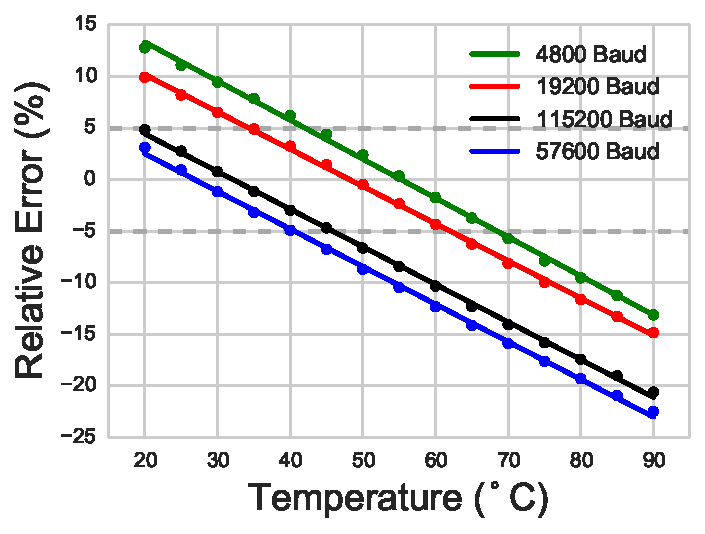
\includegraphics[width=0.5\columnwidth]{figures/baudrate_error}
    	\label{fig:baudrate_error}
    }
    \subfigure[Relative error of \acs{DCO} calibration.] {
	    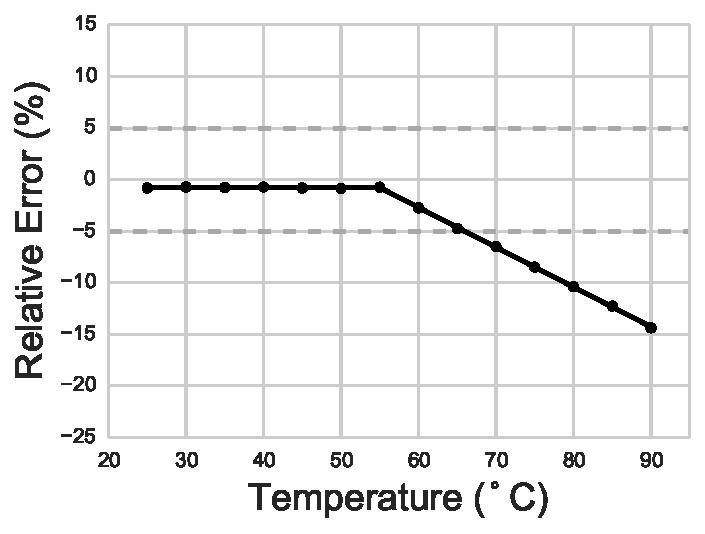
\includegraphics[width=0.5\columnwidth]{figures/reboot_dco_drift}
	    \label{fig:reboot_drift}
	}
	\subfigure[Relative error of corrected baudrate.] {
	    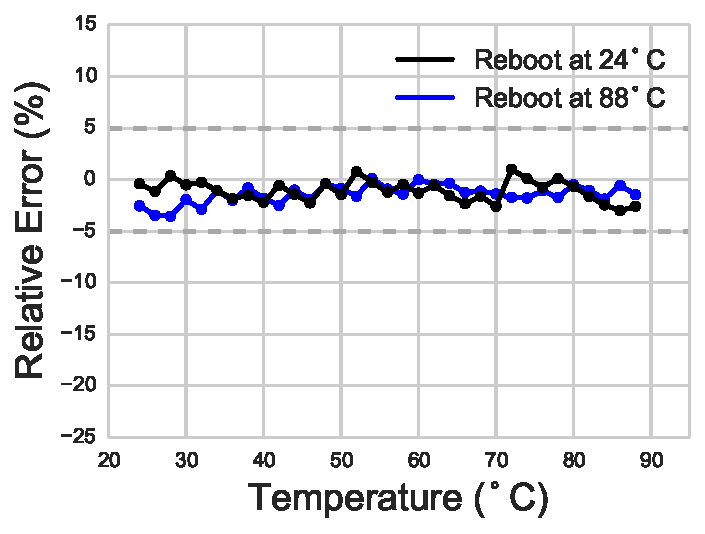
\includegraphics[width=0.5\columnwidth]{figures/baudrate_correction_error}
	    \label{fig:baudrate_look_up_error}
	}
	\subfigure[Values of baudrate correction look-up table.] {
	    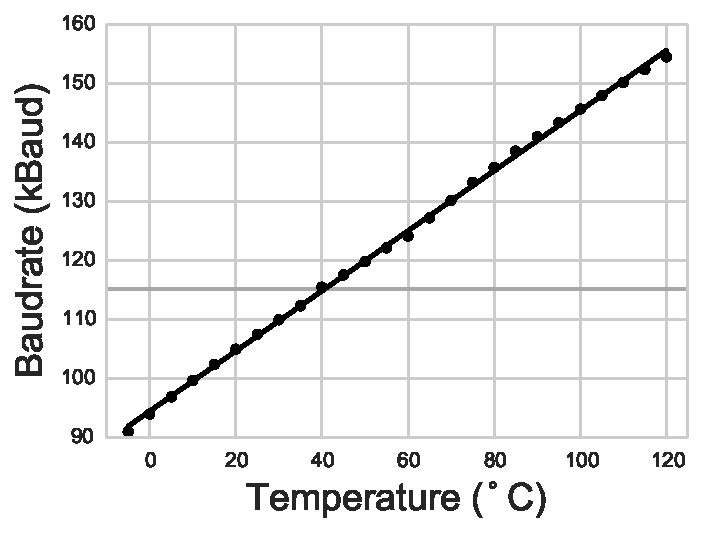
\includegraphics[width=0.5\columnwidth]{figures/baudrate_correction_table}
	    \label{fig:baudrate_look_up}
	}
	\caption{\acs{UART} and \acs{DCO} calibration errors vs. temperature. Note that \acs{UART} can tolerate up to $\pm5\%$ error.}
\end{figure}

We then measured the relative baudrate error after rebooting over temperature.
As shown in Figure~\ref{fig:reboot_drift}, the TinyOS implementation of the \ac{DCO} calibration only works until $55\,^{\circ}\mathrm{C}$, after which it has no corrective effect on CPU frequency, making periodic \ac{DCO} calibration during program execution ineffective.

We chose not to correct clock drift directly, but counteract the effect on baudrate, by creating a lookup-table of ``inverse'' correction baudrates for 115.2kbps and applying it with temperature as shown in Figure~\ref{fig:baudrate_look_up}.
Since calculation of prescaler values at runtime is costly, the look-up table contains precalculated values, which are then copied into the registers at runtime.
The on-board sensor provides temperature to the \ac{UART} module which then selects new prescaler values from the look-up table for every $5\,^{\circ}\mathrm{C}$, which shows as a sawtooth pattern in the resulting relative error of the corrected baudrate as shown in Figure~\ref{fig:baudrate_look_up_error}.

Note that the receiver can still correctly read serial data if the relative error does not deviate more than $\pm5\%$. During reception the falling edge of the startbit is used to synchronize the sampling points of all bits and with 8 databits, 1 startbit and 1 stopbit (8N1 configuration), the stopbit must be sampled during the last $10\%$ of reception time, hence an error tolerance of $\pm5\%$.
For example, the tolerance for 7-bit transfers (9 baudtimes) increases to $\pm5.56\%$.

\todo{last paragraph is a bit cryptic. Overthink it.}

\section{Bit Error Patterns}

We designed two experiments to investigate the results of Schmidt~\etal~\cite{Schmidt2013}, in particular the effect of temperature and hardware revision on bit error distribution.

\subsection{Effects of board layout}
\label{subsec:effects_of_board_layout}

While both versions we used are drop-in replacements for the Telos design devised by Polastre~\etal~\cite{Polastre2005}, the newer MTM-CM5000 version uses a slightly different schematic and different board layout.
Notable differences include the 3V voltage regulator and the layout of the radio circuitry.

In the experiment a pair of CM5000 and original motes transmitted to two CM5000 and two original motes.
This redundant placement shown in Figure~\ref{fig:8_mote_setup} was chosen so that the same transmission was received by both types.
Over the course of six days the four transmitters sent 563.500 messages each, totalling 2.254.000 transmitted messages at power setting 2. Of those transmitted messages a total of 5.280.369 messages were received, 2.497.744 of which had at least one bit error.
The experiment was located in a large climate-controlled server room in the basement, therefore the temperature remained within $20-25\,^{\circ}\mathrm{C}$ with no other changes in the environment.

\begin{figure}[H]
	\centering
	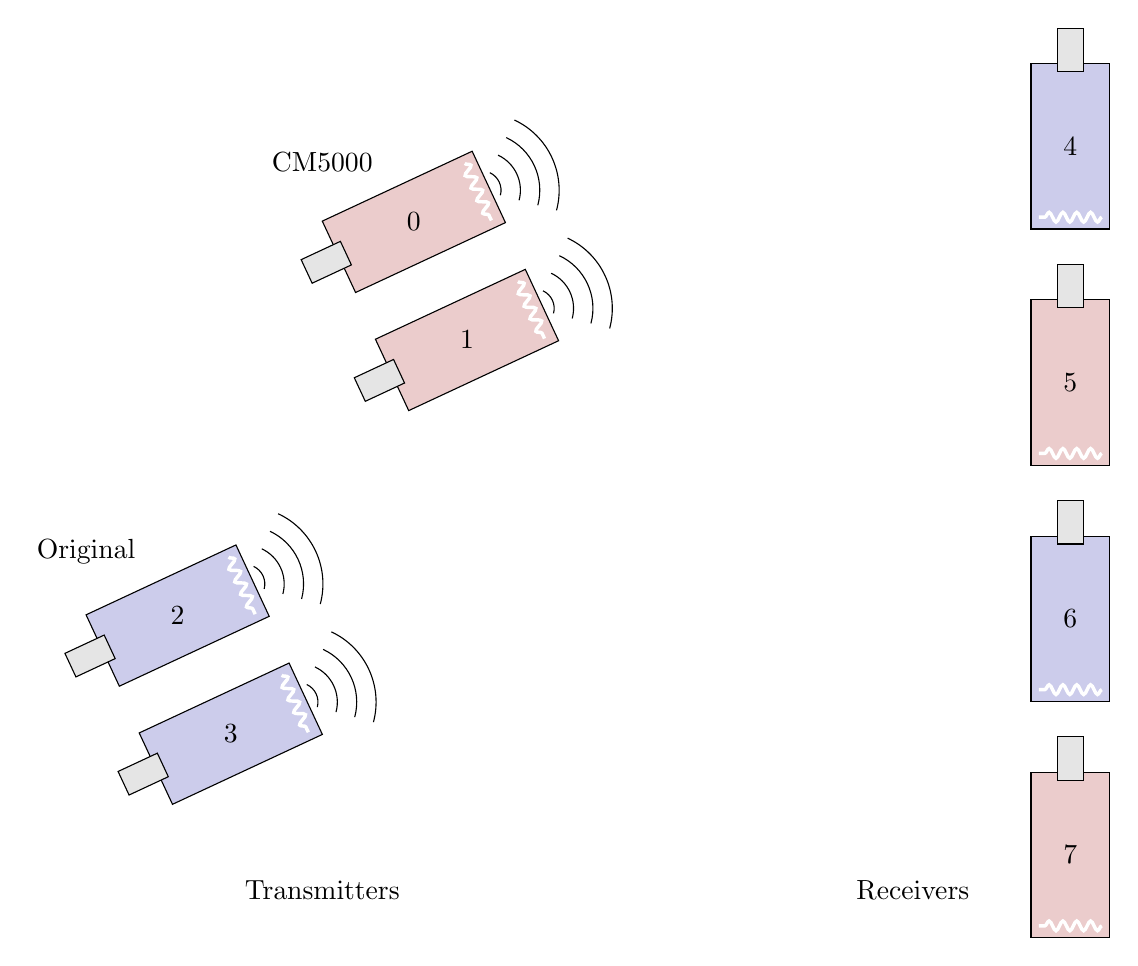
\begin{tikzpicture}
		\newcommand\receiver[5]{%
		    \begin{scope}[xshift=#1cm,yshift=#2cm,rotate=#3]
		        \draw[fill=#4] (0,0) rectangle (1,2.1);
		     	\draw[fill=black!10] (0.33,0.1) rectangle (0.66,-0.45);
		     	\draw[snake=snake, white, segment amplitude=1.75, segment length=5, line width=1.25pt] (0.1, 1.95) -- (0.9, 1.95);
		     	\node at (0.5cm, 1.05cm) {#5};
		    \end{scope}
		}
		\newcommand\transmitter[5]{%
			\receiver{#1}{#2}{#3}{#4}{#5};
		    \begin{scope}[xshift=#1cm,yshift=#2cm,rotate=#3]
		     	\draw[snake=expanding waves, segment angle=40, segment length=7] (0.5,2) -- (0.5,3);
		    \end{scope}
		}

		% new = red, old = blue
		% new transmitter
		\transmitter{3}{7}{-65}{motered}{0};
		\transmitter{3.675}{5.5}{-65}{motered}{1};		

		% new transmitter
		\transmitter{0}{2}{-65}{moteblue}{2};
		\transmitter{0.675}{0.5}{-65}{moteblue}{3};

		\receiver{13}{0}{180}{motered}{7};
		\receiver{13}{3}{180}{moteblue}{6};
		\receiver{13}{6}{180}{motered}{5};
		\receiver{13}{9}{180}{moteblue}{4};

		% labels
		\node at (3, 7.75) {CM5000};
		\node at (0, 2.8) {Original};

		\node at (3, -1.5) {Transmitters};
		\node at (10.5, -1.5) {Receivers};
	\end{tikzpicture}
	\caption{Experiment setup from above with four transmitters and receivers.}
	\label{fig:8_mote_setup}
\end{figure}

Note that the CM5000 motes required to be physically closer to the receivers at the same power setting to have similar link quality as the original motes.
This might be hinting at a difference in range between the two hardware layouts, however, our experiment was not setup to systematically investigate range.

In the initial evaluation we noted some significant differences in the quality of some links, were the co-located transmitters are sending to the same receiver.
For example, the link 3-5 is of very good quality with over 99\% PRR, however link 2-5 shows quite the opposite with less than 1\% PRR, even though both transmitters a located at the same distance and angle from the receiver.
This confirms the findings of Baccour~\etal~\cite{Baccour2012}, specifically that link quality is anisotropic, \ie the communication range exhibits a nonspherical pattern.
More exhibitions of this behavior can be found in the complete table of link qualifiers in the Appendix as Table~\ref{tab:8mote_link_qualities}.

Further analysis revealed the same bit and symbol error patterns as first discovered by Schmidt~\etal~\cite{Schmidt2013}, which state that within any transmitted symbol, the first three MSB are more likely to break than the LSB and that symbols with the MSB set to 1 (\ie 0x8 to 0xF) are more likely to brea.
The probability of bit errors are plotted in Figure~\ref{fig:8mote_bit_errors}, with the first 12 bytes (96 bits) consisting of the message header with partially fixed content and the remaining 80 bytes are the constant payload, made up of two 32 byte patterns of 0x0000, 0x1111, ..., 0xFFFF, and one 16 byte pattern of 0x00, 0x11, ..., 0xFF.

\begin{figure}[H]
	\subfigure[XL symbol influence.] {
    	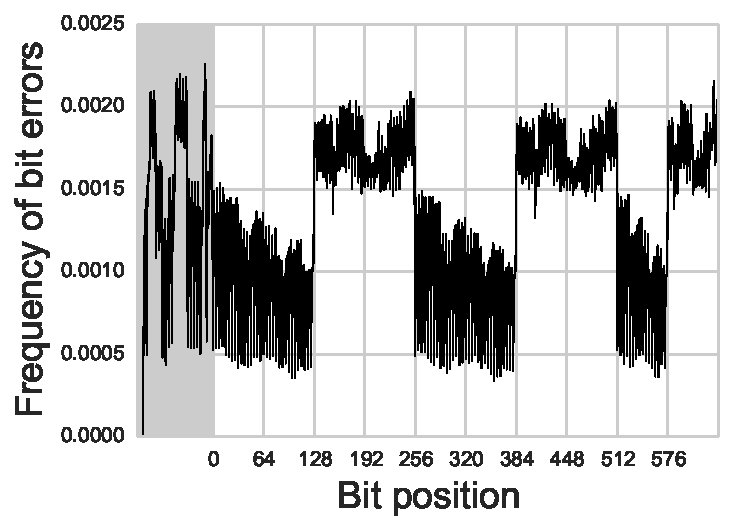
\includegraphics[width=0.5\columnwidth]{figures/8mote_0-5_xor}
    	\label{fig:8mote_bit_errors_xl}
    }
    \subfigure[L symbol influence] {
	    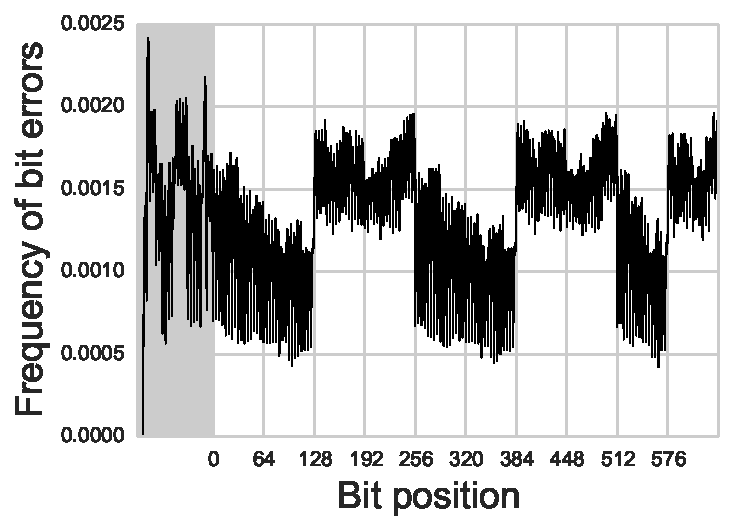
\includegraphics[width=0.5\columnwidth]{figures/8mote_1-6_xor}
	    \label{fig:8mote_bit_errors_l}
	}
	\subfigure[M influence.] {
	    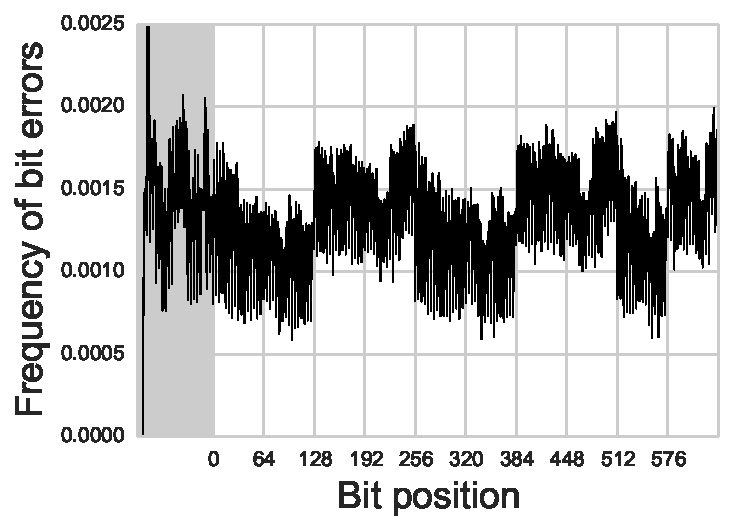
\includegraphics[width=0.5\columnwidth]{figures/8mote_2-6_xor}
	    \label{fig:8mote_bit_errors_m}
	}
	\subfigure[S influence.] {
	    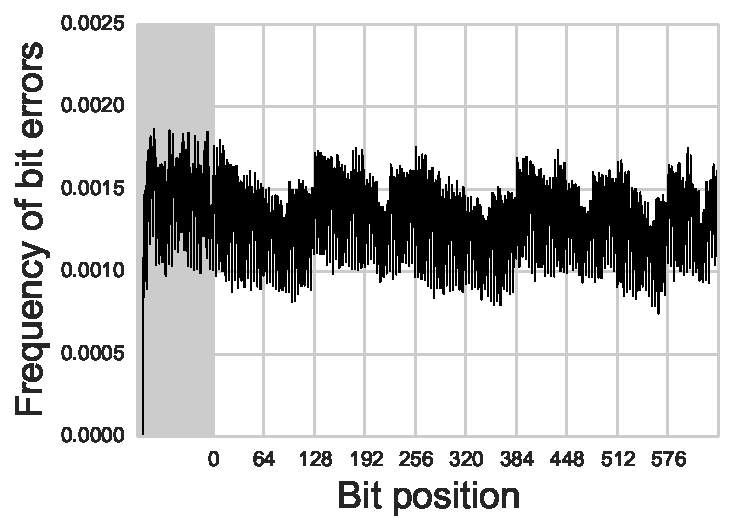
\includegraphics[width=0.5\columnwidth]{figures/8mote_2-7_xor}
	    \label{fig:8mote_bit_errors_s}
	}
	\caption{Four magnitudes of symbol content influence on bit error pattern.}
	\label{fig:8mote_bit_errors}
\end{figure}

We were able to confirm the findings of Schmidt~\etal{} and extend them with a classification of the influence of symbols on bit error probability.
The subfigures show four magnitudes of this phenomenon, ranging from and extreme to almost no difference between symbols, named XL, L, M and S.
The remaining links can be classified into these four categories as done in Table~\ref{tab:8mote_bit_error_link_classification}.

\begin{table}[H]
	\begin{tabularx}{\linewidth}{|c*{4}{|c}|}
	\hline
	\T \cellcolor{slightgray} Receiver	& \multicolumn{1}{X|}{\cellcolor{motered} \centering Sender 0} & \multicolumn{1}{X|}{\cellcolor{motered} \centering Sender 1} & \multicolumn{1}{X|}{\cellcolor{moteblue} \centering Sender 2}	& \multicolumn{1}{X|}{\cellcolor{moteblue} \centering Sender 3}\\
	\hline

	\cellcolor{moteblue}\T 4 & S  & n/a & n/a & n/a \B\\
	\hline
	\cellcolor{motered}\T  5 & XL & XL  & L   & XL  \B\\
	\hline
	\cellcolor{moteblue}\T 6 & XL & L   & M   & n/a \B\\
	\hline
	\cellcolor{motered}\T  7 & L  & n/a & S   & L   \B\\
	\hline 
	\end{tabularx}

	\caption{Classification of all links with enough bit errors (otherwise marked with n/a).}
	\label{tab:8mote_bit_error_link_classification}
\end{table}




%%%%%%%%%%%%%%%%%%%%%%%%%%%%%%%%%%%%%%%%%%%%%%%%%%%%%%%%%%%%%
%% LITERATUR UND ANDERE VERZEICHNISSE
%%%%%%%%%%%%%%%%%%%%%%%%%%%%%%%%%%%%%%%%%%%%%%%%%%%%%%%%%%%%%
%% Ein kleiner Abstand zu den Kapiteln im Inhaltsverzeichnis (toc)
\ifnotdraft{
\addtocontents{toc}{\protect\vspace*{\baselineskip}}
\cleardoublepage
%% Literaturverzeichnis
\phantomsection % phantomsection wird benötigt, damit z.B. hyperref die richtige Seite verlinkt.
\addcontentsline{toc}{chapter}{Bibliography}
%\nocite{*} %Auch nicht-zitierte BibTeX-Einträge werden angezeigt.
\bibliography{literature/literature}%Eine Datei 'literatur.bib' wird hierfür benötigt.
\bibliographystyle{acmurl}%Art der Ausgabe: plain / apalike / amsalpha / ...
}

%% Abbildungsverzeichnis
%\clearpage
%\addcontentsline{toc}{chapter}{List of Figures}
%\listoffigures

%% Tabellenverzeichnis
%\clearpage
%\addcontentsline{toc}{chapter}{List of Tables}
%\listoftables


%%%%%%%%%%%%%%%%%%%%%%%%%%%%%%%%%%%%%%%%%%%%%%%%%%%%%%%%%%%%%
%% ANHÄNGE
%%%%%%%%%%%%%%%%%%%%%%%%%%%%%%%%%%%%%%%%%%%%%%%%%%%%%%%%%%%%%
\appendix
\chapter{Appendix}

\section{List of Abbreviations}

\begin{acronym}[MOSFET]
	\setlength{\itemsep}{-\parsep}
	
	\acro{MOSFET}{Metal–Oxide–Semiconductor Field-Effect Transistor}
	\acro{ISP}{In-System Programming}
	\acro{PRR}{Packet Reception Rate}
	\acro{PID}{Proportional-Integral-Derivative}
	\acro{ATX}{Advanced Technology eXtended}
	\acro{DCO}{Digitally Controlled Oscillator}
	\acro{UART}{Universal Asynchronous Receiver Transmitter}
	\acro{BER}{Bit Error Rate}
	\acro{LQI}{Link Quality Indication}
	\acro{RSSI}{Received Signal Strength Indication}
\end{acronym}


\begin{table}
	\subtable[Average Packet Reception Rate in \%]
	{
		\begin{tabularx}{\linewidth}{|c*{4}{|d{-1}}|}
		\hline
		\T \cellcolor{slightgray} Receiver	& \multicolumn{1}{X|}{\cellcolor{motered} \centering Sender 0} & \multicolumn{1}{X|}{\cellcolor{motered} \centering Sender 1} & \multicolumn{1}{X|}{\cellcolor{moteblue} \centering Sender 2}	& \multicolumn{1}{X|}{\cellcolor{moteblue} \centering Sender 3}\\
		\hline

		\cellcolor{moteblue}\T 4 & \cellcolor{slightred} 3.2  & \cellcolor{slightgreen} 96.9 & \cellcolor{slightred} 5.5  & \cellcolor{slightgreen} 100.0 \B\\
		\hline
		\cellcolor{motered}\T 5 & 81.9 & 87.2 & \cellcolor{slightred} 0.4  & \cellcolor{slightgreen} 99.2 \B\\
		\hline
		\cellcolor{moteblue}\T 6 & \cellcolor{slightgreen} 98.1 & 75.2 & 89.9 & \cellcolor{slightred} 0.1  \B\\
		\hline
		\cellcolor{motered}\T 7 & \cellcolor{slightgreen} 96.2 & \cellcolor{slightred} 2.0    & 57.3 & 44.0	\B\\
		\hline 
		\end{tabularx}
	}

	\subtable[Average Error Free Packets Reception Rate in \%]
	{
		\begin{tabularx}{\linewidth}{|c*{4}{|d{-1}}|}
		\hline
		\T \cellcolor{slightgray} Receiver	& \multicolumn{1}{X|}{\cellcolor{motered} \centering Sender 0} & \multicolumn{1}{X|}{\cellcolor{motered} \centering Sender 1} & \multicolumn{1}{X|}{\cellcolor{moteblue} \centering Sender 2}	& \multicolumn{1}{X|}{\cellcolor{moteblue} \centering Sender 3}\\
		\hline

		\cellcolor{moteblue}\T 4 & \cellcolor{slightred} 0.0  & 69.5 & \cellcolor{slightred} 2.7  & \cellcolor{slightgreen} 100.0 \B\\
		\hline
		\cellcolor{motered}\T 5 & \cellcolor{slightred} 7.1 & 10.8 & \cellcolor{slightred} 0.0  & 88.3 \B\\
		\hline
		\cellcolor{moteblue}\T 6 & 83.8 & \cellcolor{slightred} 2.1 & 22.1 & \cellcolor{slightred} 0.0  \B\\
		\hline
		\cellcolor{motered}\T 7 & \cellcolor{slightgreen} 96.0 & \cellcolor{slightred} 0.1    & \cellcolor{slightred} 9.8 & \cellcolor{slightred} 1.4	\B\\
		\hline 
		\end{tabularx}
	}

	\subtable[Average LQI values]
	{
		\begin{tabularx}{\linewidth}{|c*{4}{|d{-1}}|}
		\hline
		\T \cellcolor{slightgray} Receiver	& \multicolumn{1}{X|}{\cellcolor{motered} \centering Sender 0} & \multicolumn{1}{X|}{\cellcolor{motered} \centering Sender 1} & \multicolumn{1}{X|}{\cellcolor{moteblue} \centering Sender 2}	& \multicolumn{1}{X|}{\cellcolor{moteblue} \centering Sender 3}\\
		\hline

		\cellcolor{moteblue}\T 4 & \cellcolor{slightred} 50 & 79 & \cellcolor{slightred} 77 & \cellcolor{slightgreen} 101 \B\\
		\hline
		\cellcolor{motered}\T 5 & 71 & 72 & \cellcolor{slightred} 49  & 87 \B\\
		\hline
		\cellcolor{moteblue}\T 6 & 85 & 67 & 73 & \cellcolor{slightred} 35  \B\\
		\hline
		\cellcolor{motered}\T 7 & \cellcolor{slightgreen} 106 & \cellcolor{slightred} \cellcolor{slightred} 44 & 65 & 61	\B\\
		\hline 
		\end{tabularx}
	}

	\caption{Complete table of link qualifiers from the experiment described in Subsection~\ref{subsec:effects_of_board_layout}. Good links (PRR > 90\%) are marked green, bad links (PRR < 10\%) red. Notice the distinction between PRR in Table (a) and \emph{error-free} PRR in Table (b) in comparison to LQI in Table (c).}

	\label{tab:8mote_link_qualities}
\end{table}

\end{document}
